\documentclass[12pt]{article}
\usepackage{amsmath}
\usepackage{amssymb}
\usepackage{geometry}
\usepackage{enumerate}
\usepackage{natbib}
\usepackage{float}%稳定图片位置
\usepackage{graphicx}%画图
\usepackage[english]{babel}
\usepackage{a4wide}
\usepackage{indentfirst}%缩进
\usepackage{enumerate}%加序号
\usepackage{multirow}%合并行
\usepackage{tikz}%图
\title{\large UM-SJTU JOINT INSTITUTE\\DISCRETE MATHEMATICS\\(VE203)\\\ \\\ \\\ \\\ \\\ \\\ \\\ \\\ \\\ \\\ \\\
ASSIGNMENT 9\\\ \\\ \\\ \\\ \\\ \\\ }
\author{Name: Pan Chongdan\\ID: 516370910121}
\date{Date: \today}


\begin{document}
\maketitle
\newpage
\section{Q1}
\begin{enumerate}[(i)]
\item
The sequence is (0,4,9,27,$\cdots$)
\\So the formula
\begin{eqnarray}g(n)=
\begin{cases}
0,n=1\cr 4,n=2 \cr 3^{n-1},n\ge 3\end{cases}
\end{eqnarray}
\item
The sequence is (0,0,3,0,$\frac{9}{2},\cdots$)
\\So the formula
\begin{eqnarray}g(n)=
\begin{cases}
0,n=1\vee n\mathrm{\quad is\quad even} \cr \frac{3^{n-2}}{(n-2)!},n=2k+1,k\in\mathbb{Z^+}\end{cases}
\end{eqnarray}
\item
The sequence is (0,1,-1,0,$\cdots$)
\\So the formula
\begin{eqnarray}g(n)=
\begin{cases}
0,n=3k\cr 1,n=3k+1 \cr -1,n=3k+2,k\in\mathbb{Z}\end{cases}
\end{eqnarray}
\end{enumerate}
\section{Q2}
\begin{figure}[H]
\centering
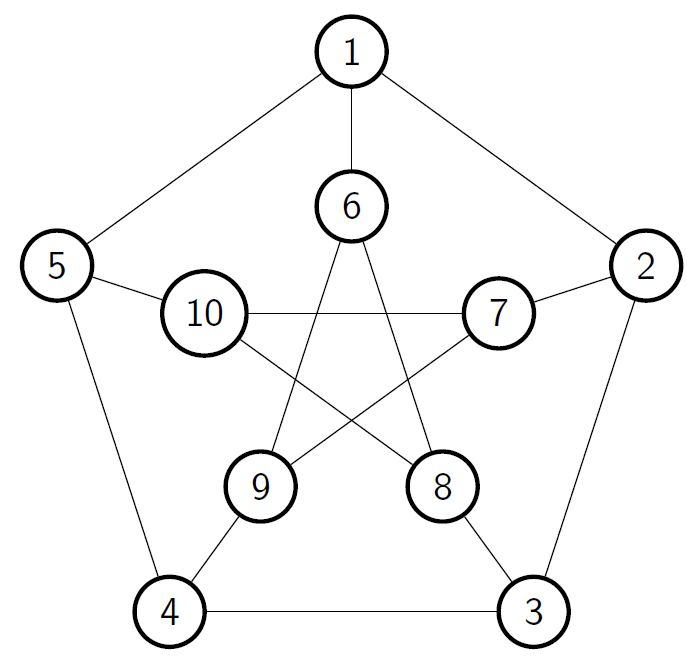
\includegraphics[scale=0.3]{P1.jpg}
\caption{Petersen Graph}
\end{figure} 
Since the degree of all vertex is 3, and we can only get in and out of one vertex once, so every vertex must have exactly two edges in the Hamilton circuit, assume there exists a Hamilton circuit $E_H$ includes all the edges of the Hamilton circuit.
\begin{enumerate}
\item If $\{1,2\}\notin E_H\Rightarrow\{1,5\},\{1,6\},\{2,7\},\{2,3\}\in E_H$
\begin{enumerate}[(a)]
\item Then if $\{3,8\}\in E_H\Rightarrow\{4,9\},\{5,4\}\in E_H\Rightarrow\{10,8\},\{10,7\}\in E_H\Rightarrow\{9,6\}\in E_H.$ So the circuit become $\{1\rightarrow5\rightarrow4\rightarrow9\rightarrow6\rightarrow1\}$, which doesn't pass every vertex. 
\item If $\{3,4\}\in E_H\Rightarrow\{8,10\},\{8,6\}\in E_H\Rightarrow\{9,4\},\{9,7\}\in E_H\Rightarrow\{10,5\}\in E_H.$ So the circuit become $\{1\rightarrow5\rightarrow10\rightarrow8\rightarrow6\rightarrow1\}$, which also doesn't pass every vertex. 
\end{enumerate}
\item If $\{1,6\}\notin E_H\Rightarrow\{1,5\},\{1,2\},\{6,9\},\{6,8\}\in E_H$
\begin{enumerate}[(a)]
\item Then if $\{5,4\}\in E_H\Rightarrow\{10,8\},\{10,7\}\in E_H\Rightarrow\{3,2\},\{3,4\}\in E_H\Rightarrow\{3,6\}\in E_H.$ So the circuit become $\{1\rightarrow5\rightarrow4\rightarrow3\rightarrow2\rightarrow1\}$, which doesn't pass every vertex. 
\item If $\{5,10\}\in E_H\Rightarrow\{4,9\},\{4,3\}\in E_H\Rightarrow\{7,10\},\{7,2\}\in E_H.$ So the circuit become $\{1\rightarrow5\rightarrow10\rightarrow7\rightarrow2\rightarrow1\}$, which also doesn't pass every vertex. 
\end{enumerate}
\end{enumerate}
So we can never find a Hamilton circuit passing through vertex 1.
\par If we cut vertex 1 from the Graph then the circuit can be $\{2\rightarrow3\rightarrow4\rightarrow5\rightarrow10\rightarrow8\rightarrow6\rightarrow9\rightarrow7\rightarrow2\}$
\par If we cut vertex 6 from the Graph then the circuit can be $
\{1\rightarrow2\rightarrow7\rightarrow9\rightarrow4\rightarrow3\rightarrow8\rightarrow10\rightarrow5\rightarrow1\}$
\section{Q3}
Yes
\begin{figure}[H]
\centering
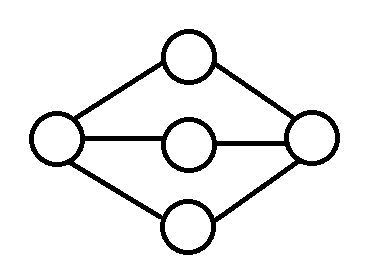
\includegraphics[scale=0.3]{P5.jpg}
\caption{The graph doesn't have a Hamilton circuit}
\end{figure} 
\section{Q4}
\begin{enumerate}[(i)]
\item 
Yes
\begin{figure}[H]
\centering
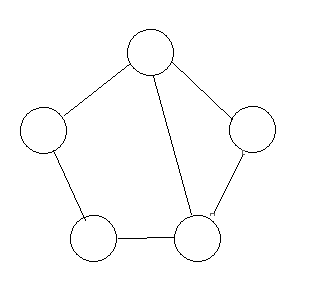
\includegraphics[scale=0.5]{P2.jpg}
\end{figure}
\item
No, since there are two vertexes whose degrees are 4, then there can't exist a vertex with degree=1
\item
Yes
\begin{figure}[H]
\centering
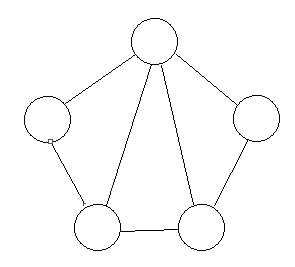
\includegraphics[scale=0.5]{P3.jpg}
\end{figure}
\item
No, because the sum must be even
\end{enumerate}
\section{Q5}
It's clear that for a graph whose order is $n$ and only has one connected components, it's minimal size is $e\ge n$. If we break it into to connected two components, we must cut off at least one wedge $\therefore e_1\ge e-1\ge n-1$. Similarly, if we break it into $n$ connected components, we must cut off at least $k$ wedge $\therefore e_k\ge e-k\ge n-k\Rightarrow k\ge n-e_k $
\section{Q6}
The least number is 3
\begin{figure}[H]
\centering
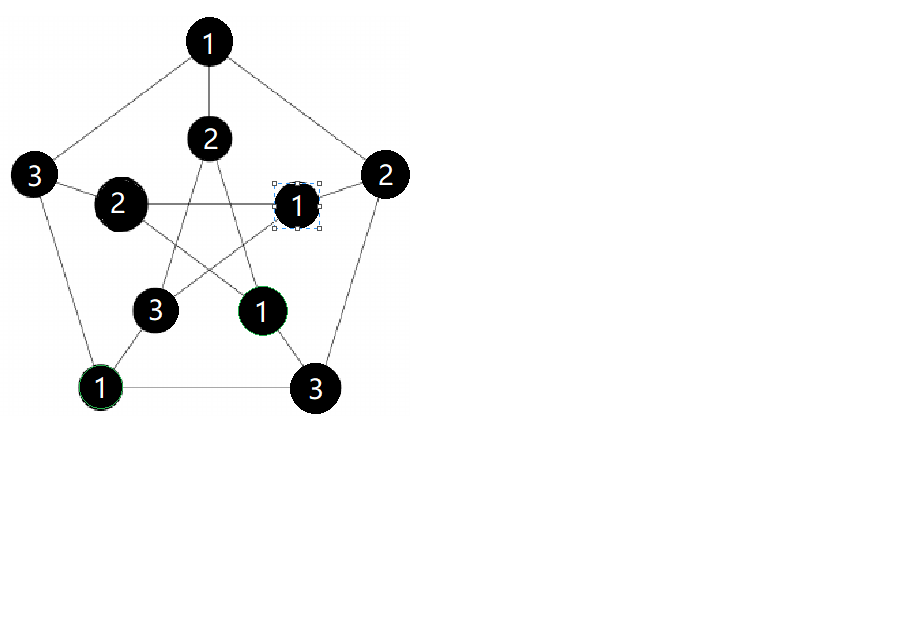
\includegraphics[scale=0.5]{P4.jpg}
\end{figure} 
\section{Q7}
\begin{enumerate}[(i)]
\item Assume $V=\{v_1,v_2\cdots,v_n\}$ and $\forall e=\{v_a,v_b\}\in E$. 
\\Let $X$ be the set of all sets containing two elements of $\mathbb{N}$
\par For example, if $G=(V,E),V=\{1,2,3,4\},E=\{\{1,2\},\{1,3\},\{1,4\},\{2,3\},\{3,4\}\}$
\\$X=\{\{1,2\},\{1,3\},\{1,4\}\cdots\{3,4\}\cdots\}$. According to $G$, we know that vertex 1 is connected to vertex 2,3,4
,so we use $\{\{1,2\},\{1,3\},\{1,4\}\}$ to donate the bijection of vertex 1. Similarly $\{\{1,2\},\{2,3\}\}$ can donate vertex 2. All these donation can form $\chi$ which is a subset of $P(X)$ Then $\{x,y\}=\{\{\{1,2\},\{1,3\},\{1,4\}\},\{\{1,2\},\{2,3\}\}\}\in E_{\chi}$ can donate the wedge. $\therefore H\cong G_{\chi}$   
\item In the last example $|X|=3+2+1=6,n=\frac{n(n-1)}{2}=\frac{n^2-n}{2}$
\end{enumerate}
\section{Q8}
\begin{enumerate}[(i)]
\item $$f(n)a_n=g(n)a_{n-1}+h(n)$$
$$Q(n)f(n)a_n=b_{n-1}+Q(n)h(n)$$
$$Q(n)f(n)=\frac{f(1)f(2)\cdots f(n)}{g(1)g(2)\cdots g(n+1)}g(n+1)=g(n+1)Q(n+1)$$
$$\therefore b_n=b_{n+1}+Q(n)h(n)$$
\item 
$$b_0=g(1)Q(1)C\Rightarrow b_n=g(1)Q(1)C+\sum_{i=1}^nQ(i)h(i)$$
$$a_n=\frac{b_n}{g(n+1)Q(n+1)},Q(1)=\frac{1}{g(1)}$$
$$\therefore a_n=\frac{C+\sum_{i=1}^nQ(i)h(i)}{g(n+1)Q(n+1)}$$
\item 
$$C=1,f(n)=1,h(n)=n,g(n)=n+3$$
$$Q(n)=\frac{6}{(n+3)!}$$
$$a_n=\frac{1+\sum_{i=1}^n\frac{6n}{(n+3)!}}{\frac{6(n+4)}{(n+4)!}}=\frac{(n+3)!+(n+3)!\sum_{i=1}^n\frac{6n}{(n+3)!}}{6}$$
\end{enumerate}
\end{document}